\documentclass{standalone}
\usepackage{tikz}
\usetikzlibrary{patterns, positioning}
\usepackage[sfdefault]{ClearSans} %% option 'sfdefault' activates Clear Sans as the default text font
\usepackage[T1]{fontenc}

\begin{document}
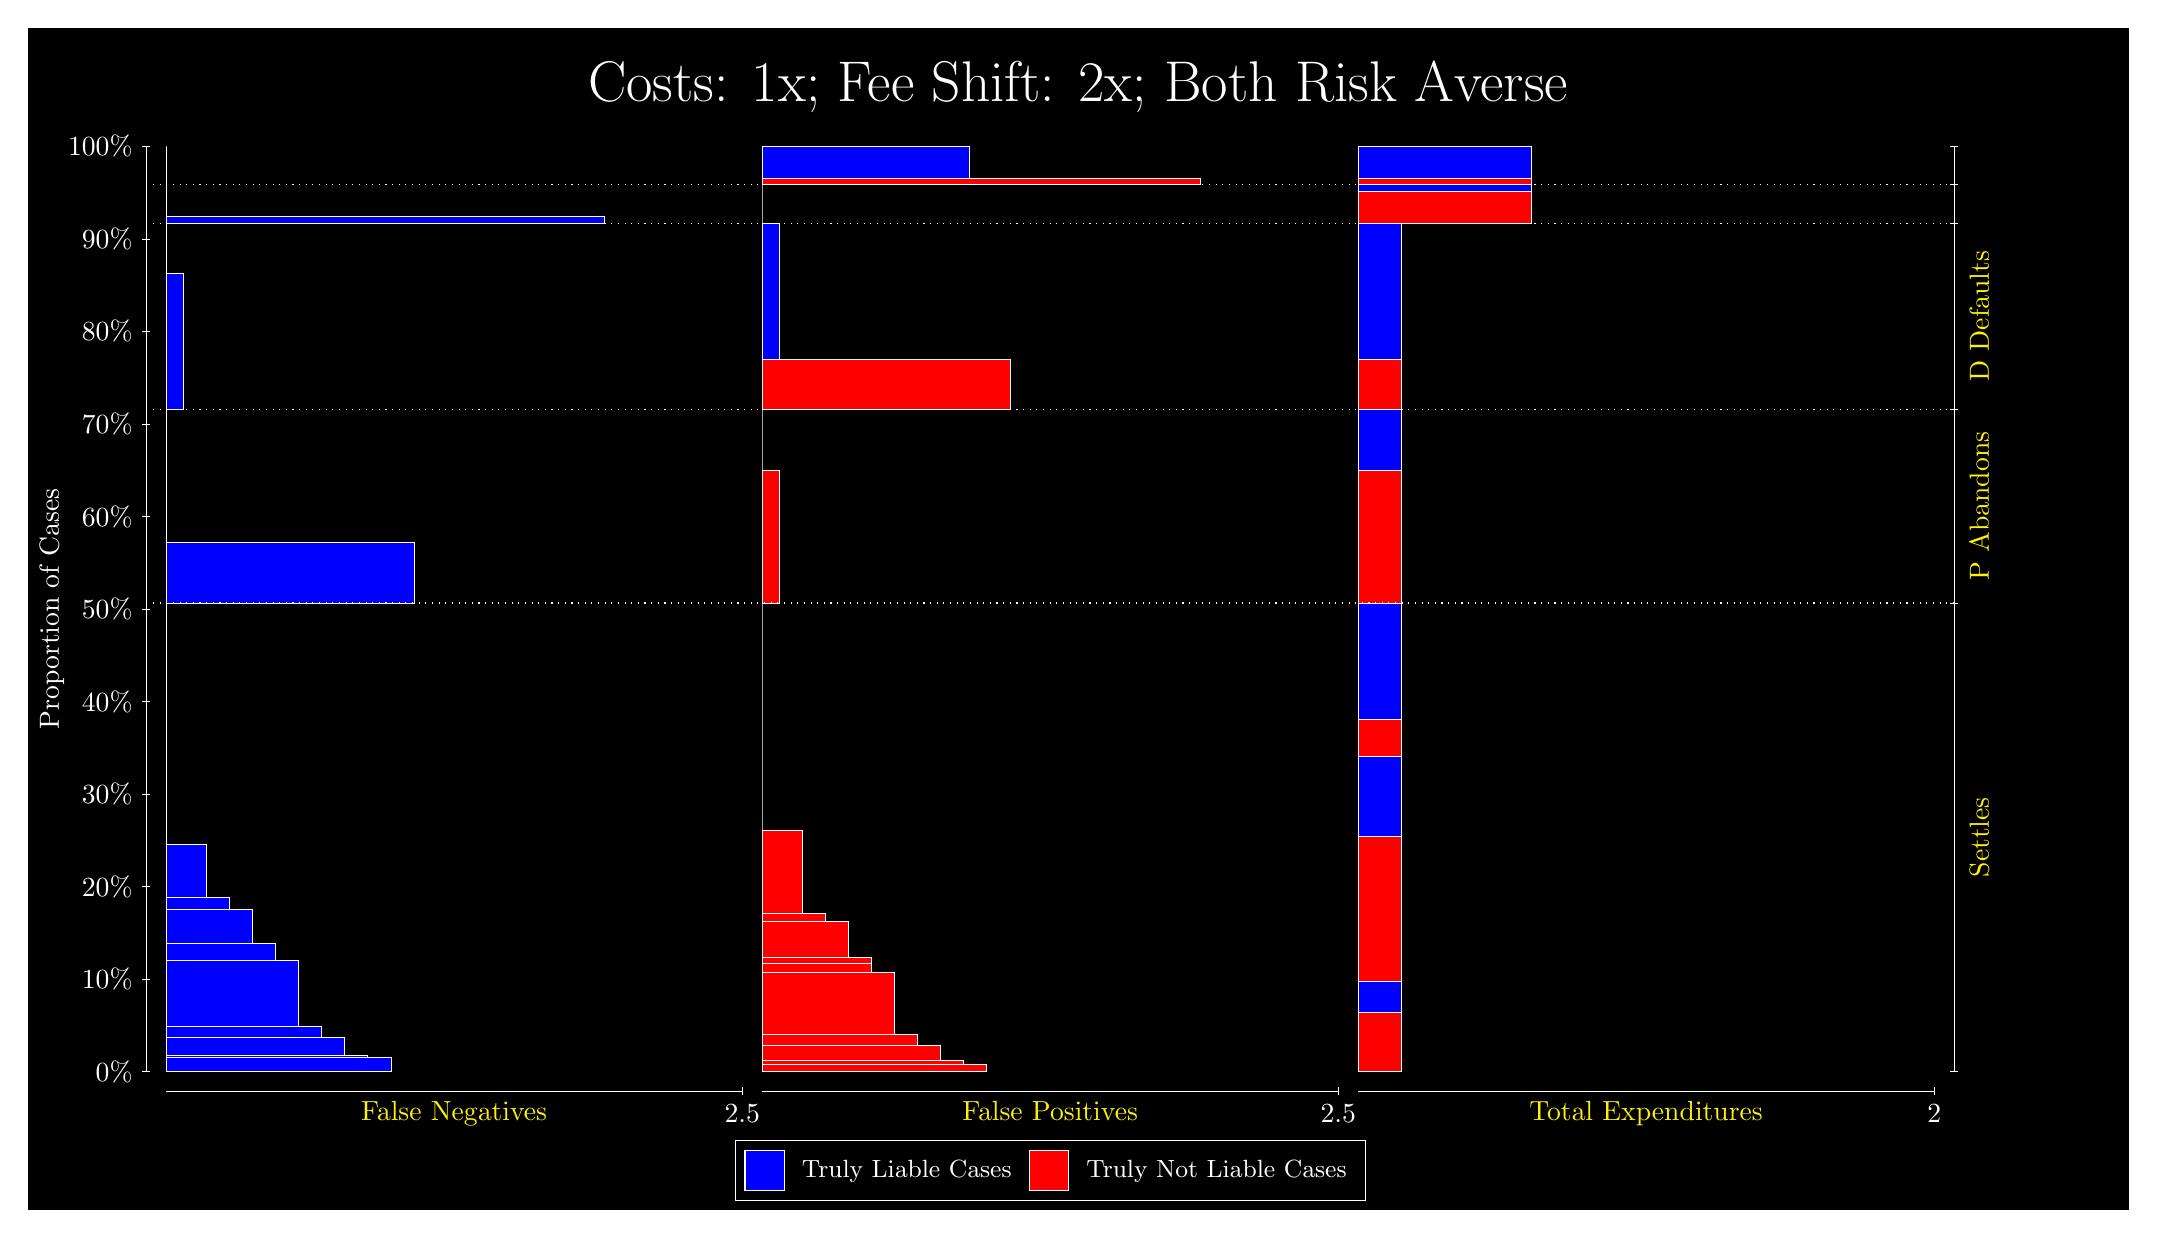
\begin{tikzpicture}
\draw[fill=black] (0,0) rectangle (26.667,15);
\draw[text=white] (0,13.5) rectangle (26.667,15) node[midway] {\huge Costs: 1x; Fee Shift: 2x; Both Risk Averse};
\draw[white, very thin] (1.5,1.75) -- (1.5,13.5);
\node[rotate=90, text=white, anchor=center] at (0.3, 7.625) {Proportion of Cases};
\draw[white, very thin] (1.45,1.75) -- (1.55,1.75);
\node[text=white, anchor=east] at (1.45, 1.75) {0\%};
\draw[white, very thin] (1.45,2.925) -- (1.55,2.925);
\node[text=white, anchor=east] at (1.45, 2.925) {10\%};
\draw[white, very thin] (1.45,4.1) -- (1.55,4.1);
\node[text=white, anchor=east] at (1.45, 4.1) {20\%};
\draw[white, very thin] (1.45,5.275) -- (1.55,5.275);
\node[text=white, anchor=east] at (1.45, 5.275) {30\%};
\draw[white, very thin] (1.45,6.45) -- (1.55,6.45);
\node[text=white, anchor=east] at (1.45, 6.45) {40\%};
\draw[white, very thin] (1.45,7.625) -- (1.55,7.625);
\node[text=white, anchor=east] at (1.45, 7.625) {50\%};
\draw[white, very thin] (1.45,8.8) -- (1.55,8.8);
\node[text=white, anchor=east] at (1.45, 8.8) {60\%};
\draw[white, very thin] (1.45,9.975) -- (1.55,9.975);
\node[text=white, anchor=east] at (1.45, 9.975) {70\%};
\draw[white, very thin] (1.45,11.15) -- (1.55,11.15);
\node[text=white, anchor=east] at (1.45, 11.15) {80\%};
\draw[white, very thin] (1.45,12.325) -- (1.55,12.325);
\node[text=white, anchor=east] at (1.45, 12.325) {90\%};
\draw[white, very thin] (1.45,13.5) -- (1.55,13.5);
\node[text=white, anchor=east] at (1.45, 13.5) {100\%};

\draw[white, very thin] (24.457,1.75) -- (24.457,13.5);
\draw[white, very thin] (24.407,1.75) -- (24.507,1.75);
\node[anchor=west] at (24.407, 1.75) {};
\draw[white, very thin] (24.407,7.7003) -- (24.507,7.7003);
\node[anchor=west] at (24.407, 7.7003) {};
\draw[white, very thin] (24.407,10.161) -- (24.507,10.161);
\node[anchor=west] at (24.407, 10.161) {};
\draw[white, very thin] (24.407,12.525) -- (24.507,12.525);
\node[anchor=west] at (24.407, 12.525) {};
\draw[white, very thin] (24.407,13.015) -- (24.507,13.015);
\node[anchor=west] at (24.407, 13.015) {};
\draw[white, very thin] (24.407,13.5) -- (24.507,13.5);
\node[anchor=west] at (24.407, 13.5) {};

\draw[white, very thin, fill=blue] (1.75,1.75) rectangle (4.6044,1.9281);
\draw[white, very thin, fill=blue] (1.75,1.9281) rectangle (4.3116,1.9624);
\draw[white, very thin, fill=blue] (1.75,1.9624) rectangle (4.0188,2.1835);
\draw[white, very thin, fill=blue] (1.75,2.1835) rectangle (3.7261,2.3249);
\draw[white, very thin, fill=blue] (1.75,2.3249) rectangle (3.4333,3.1628);
\draw[white, very thin, fill=blue] (1.75,3.1628) rectangle (3.1406,3.3801);
\draw[white, very thin, fill=blue] (1.75,3.3801) rectangle (2.8478,3.812);
\draw[white, very thin, fill=blue] (1.75,3.812) rectangle (2.5551,3.9647);
\draw[white, very thin, fill=blue] (1.75,3.9647) rectangle (2.2623,4.6369);
\draw[white, very thin, fill=red] (1.75,4.6369) rectangle (1.75,7.7003);
\draw[white, very thin, fill=blue] (1.75,7.7003) rectangle (4.8971,8.4762);
\draw[white, very thin, fill=red] (1.75,8.4762) rectangle (1.75,10.161);
\draw[white, very thin, fill=blue] (1.75,10.161) rectangle (1.9696,11.888);
\draw[white, very thin, fill=red] (1.75,11.888) rectangle (1.75,12.525);
\draw[white, very thin, fill=blue] (1.75,12.525) rectangle (7.3123,12.609);
\draw[white, very thin, fill=red] (1.75,12.609) rectangle (1.75,13.015);
\draw[white, very thin, fill=red] (1.75,13.015) rectangle (1.75,13.098);
\draw[white, very thin, fill=blue] (1.75,13.098) rectangle (1.75,13.5);
\draw[white, very thin, fill=red] (9.3189,1.75) rectangle (12.173,1.8358);
\draw[white, very thin, fill=red] (9.3189,1.8358) rectangle (11.88,1.888);
\draw[white, very thin, fill=red] (9.3189,1.888) rectangle (11.588,2.0844);
\draw[white, very thin, fill=red] (9.3189,2.0844) rectangle (11.295,2.218);
\draw[white, very thin, fill=red] (9.3189,2.218) rectangle (11.002,3.0119);
\draw[white, very thin, fill=red] (9.3189,3.0119) rectangle (10.709,3.1276);
\draw[white, very thin, fill=red] (9.3189,3.1276) rectangle (10.709,3.1997);
\draw[white, very thin, fill=red] (9.3189,3.1997) rectangle (10.417,3.6632);
\draw[white, very thin, fill=red] (9.3189,3.6632) rectangle (10.124,3.7644);
\draw[white, very thin, fill=red] (9.3189,3.7644) rectangle (9.8312,4.8134);
\draw[white, very thin, fill=blue] (9.3189,4.8134) rectangle (9.3189,7.7003);
\draw[white, very thin, fill=red] (9.3189,7.7003) rectangle (9.5384,9.3851);
\draw[white, very thin, fill=blue] (9.3189,9.3851) rectangle (9.3189,10.161);
\draw[white, very thin, fill=red] (9.3189,10.161) rectangle (12.466,10.799);
\draw[white, very thin, fill=blue] (9.3189,10.799) rectangle (9.5384,12.525);
\draw[white, very thin, fill=red] (9.3189,12.525) rectangle (9.3189,12.932);
\draw[white, very thin, fill=blue] (9.3189,12.932) rectangle (9.3189,13.015);
\draw[white, very thin, fill=red] (9.3189,13.015) rectangle (14.881,13.098);
\draw[white, very thin, fill=blue] (9.3189,13.098) rectangle (11.954,13.5);
\draw[white, very thin, fill=red] (16.888,1.75) rectangle (17.437,2.5025);
\draw[white, very thin, fill=blue] (16.888,2.5025) rectangle (17.437,2.8993);
\draw[white, very thin, fill=red] (16.888,2.8993) rectangle (17.437,4.7422);
\draw[white, very thin, fill=blue] (16.888,4.7422) rectangle (17.437,5.7582);
\draw[white, very thin, fill=red] (16.888,5.7582) rectangle (17.437,6.2262);
\draw[white, very thin, fill=blue] (16.888,6.2262) rectangle (17.437,7.7003);
\draw[white, very thin, fill=red] (16.888,7.7003) rectangle (17.437,9.3851);
\draw[white, very thin, fill=blue] (16.888,9.3851) rectangle (17.437,10.161);
\draw[white, very thin, fill=red] (16.888,10.161) rectangle (17.437,10.799);
\draw[white, very thin, fill=blue] (16.888,10.799) rectangle (17.437,12.525);
\draw[white, very thin, fill=red] (16.888,12.525) rectangle (19.083,12.932);
\draw[white, very thin, fill=blue] (16.888,12.932) rectangle (19.083,13.015);
\draw[white, very thin, fill=red] (16.888,13.015) rectangle (19.083,13.098);
\draw[white, very thin, fill=blue] (16.888,13.098) rectangle (19.083,13.5);
\draw[white, dotted] (1.5,7.7003) -- (24.457,7.7003);
\draw[white, dotted] (1.5,10.161) -- (24.457,10.161);
\draw[white, dotted] (1.5,12.525) -- (24.457,12.525);
\draw[white, dotted] (1.5,13.015) -- (24.457,13.015);
\draw[white, very thin] (1.75,1.5) -- (9.0689,1.5);
\node[text=yellow, anchor=north] at (5.4094, 1.5) {False Negatives};
\draw[white, very thin] (9.0689,1.45) -- (9.0689,1.55);
\node[text=white, anchor=north] at (9.0689, 1.45) {2.5};

\draw[white, very thin] (9.3189,1.5) -- (16.638,1.5);
\node[text=yellow, anchor=north] at (12.978, 1.5) {False Positives};
\draw[white, very thin] (16.638,1.45) -- (16.638,1.55);
\node[text=white, anchor=north] at (16.638, 1.45) {2.5};

\draw[white, very thin] (16.888,1.5) -- (24.207,1.5);
\node[text=yellow, anchor=north] at (20.547, 1.5) {Total Expenditures};
\draw[white, very thin] (24.207,1.45) -- (24.207,1.55);
\node[text=white, anchor=north] at (24.207, 1.45) {2};

\node[text=yellow, centered, rotate=90] at (24.777, 4.7252) {Settles};
\node[text=yellow, centered, rotate=90] at (24.777, 8.9307) {P Abandons};
\node[text=yellow, centered, rotate=90] at (24.777, 11.343) {D Defaults};



\draw (12.978300999999998,1.5) node[draw=none] (baseCoordinate) {};
\begin{scope}[align=center]
        \matrix[scale=0.5, draw=white, below=0.5cm of baseCoordinate, nodes={draw}, column sep=0.1cm]{
            \node[rectangle, draw, minimum width=0.5cm, minimum height=0.5cm, fill=blue] {}; &
            \node[draw=none, font=\small, text=white] (B) {Truly Liable Cases}; &
            \node[rectangle, draw, minimum width=0.5cm, minimum height=0.5cm, fill=red] {}; &
            \node[draw=none, font=\small, text=white] (B) {Truly Not Liable Cases}; \\
            };
\end{scope}

\end{tikzpicture}
\end{document}